\chapter{Operating Mechanism}
\section{Teakwood Working Flow}
So far we've already known that Teakwood follows a "MTV" design pattern and has a loosely coupling design. We also know that Teakwood uses python object to work with database by mapping. Plus, Teakwood template language is powerful for generating HTML files. Now let's join all these feathers to see how Teakwood process a request from user. \\

\begin{figure}[h]
\centering
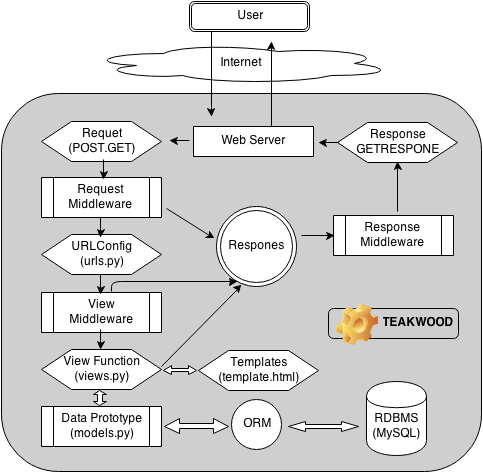
\includegraphics[scale=0.5]{./http_request_response}
\caption{Teakwood Request-Response Working Flow}
\label{fig:label} % insert suitable label, this is used to refer to a fig from within the text as shown above
\end{figure}
Then, let's put it in real world to see how this structure works. For example, a user want to view all the job status under his/her account.\\
$\bullet$ Click the job functional button.\\
$\bullet$ Button triggers a request.\\
$\bullet$ Request goes to request middleware for identity check, if legal? auth?\\
$\bullet$ if yes, goes to response and raised an error page;\\
$\bullet$ if no, goes to urlconfig to locate the right URL.\\
$\bullet$ URL goes to view middleware for legibility check, if wrong URL, auth?\\
$\bullet$ if yes, goes to response and raises an error page;\\
$\bullet$ if no, goes to view function. \\
$\bullet$ View function check if need data? if need template?\\
$\bullet$ if need data, trigger models to fetch data from database;\\
$\bullet$ if need template, find the right template, also fetch css, js and imgs.\\
$\bullet$ Send all files to response and rendering web page.\\
$\bullet$ Display the final page to user.



